\section{Move Semantics}

% TODO: finish slide
\begin{frame}[fragile]{Object Model Revision}
  C++ object lifecycle:
  \begin{itemize}
    \item Objects can be constructed in some storage location (their lifetime begins).
    \item When a destructor is called at that storage location, the lifetime ends.
  \end{itemize}

  For stack allocated objects:
  \begin{itemize}
    \item Storage location is known at compile time (offset within stack frame).
    \item Lifetime is known at compile time (when the scope ends).
    \begin{itemize}
      \item Lifetime begins when the constructor is called on the storage location.
      \item Compiler generates calls to the destructor at the end of the scope.
    \end{itemize}
  \end{itemize}
\end{frame}

% TODO: finish this slide
\begin{frame}[fragile]{Construction}
  Constructors and methods implicitly take the \emph{address of the object} as an argument 
  (binds to the argument \verb|this|, which is passed through register \verb|rdi|).

\end{frame}

\begin{frame}[fragile]{Compilation Example}
  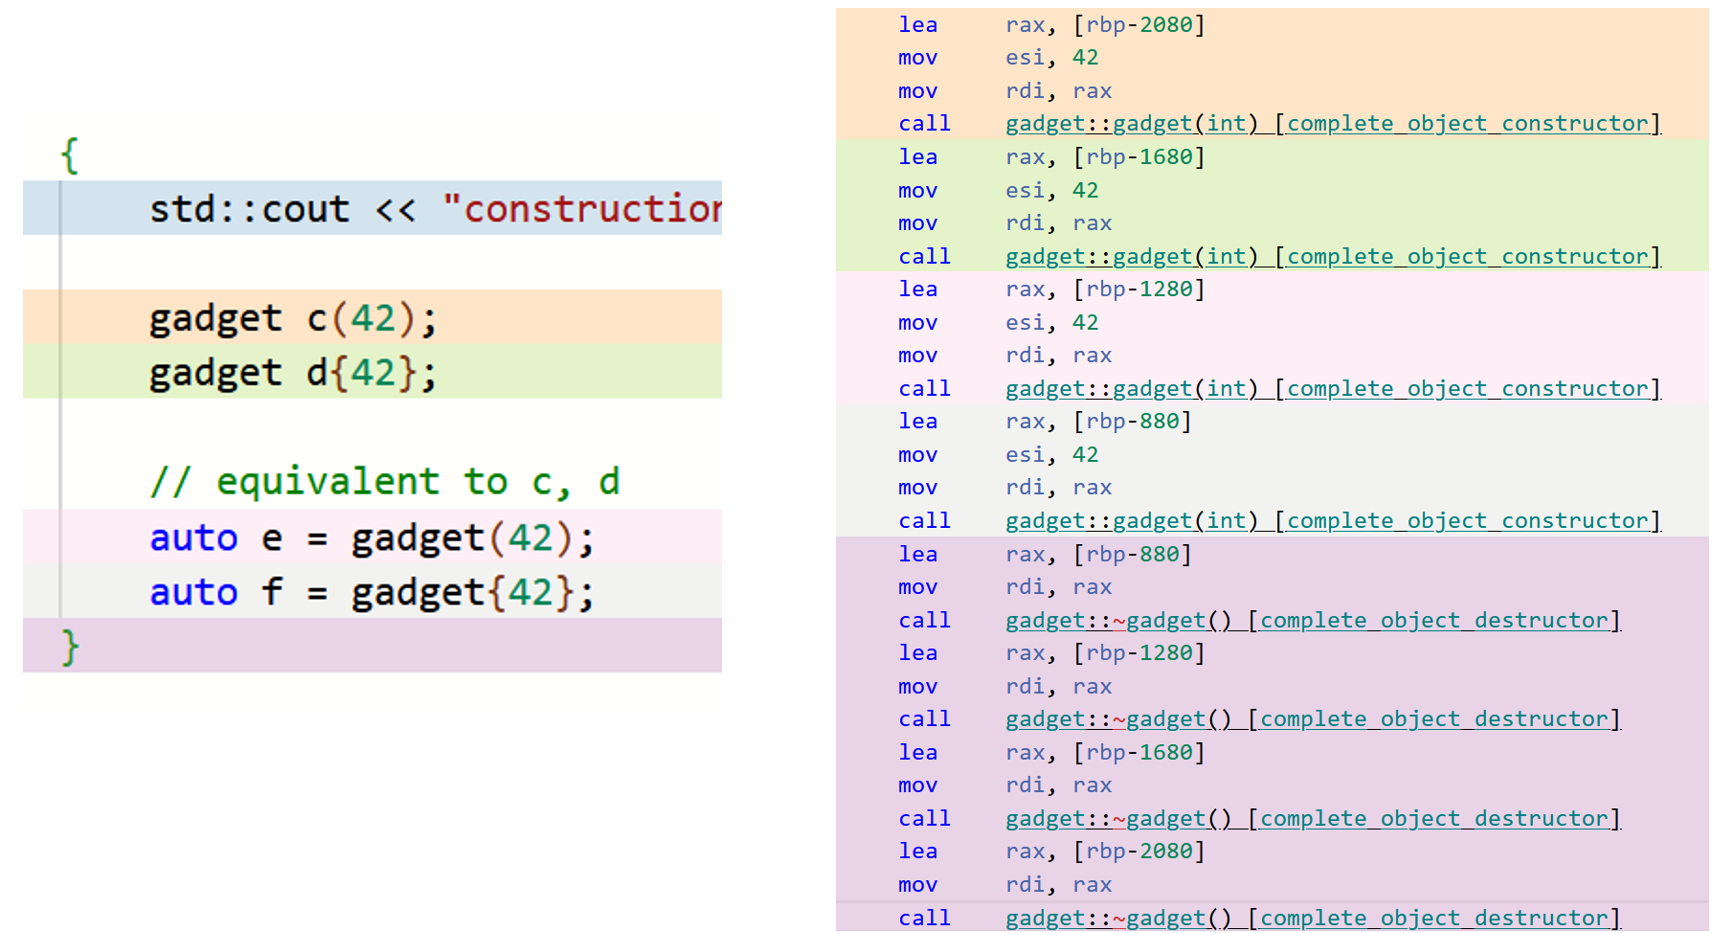
\includegraphics[width=12cm]{assets/constructor_compiled.png}
\end{frame}

% TODO: finish this slide
\begin{frame}[fragile]{Placement New}
  \begin{sqt:definition}
    \emph{Non-allocating placement} (known colloquially as \emph{placement new}) allows
    you to construct an object in a specified memory location of the programmer's choosing.
  \end{sqt:definition}

  \begin{minted}{cpp}
    // calls the constructor gadget::gadget() on address 123456
    new ((void *) 123456) gadget{};
  \end{minted}

  The lifetime of the resulting object is NOT automatic.
  Thus it is the responsibility of the programmer to call the destructor to end lifetime.

  \begin{minted}{cpp}
    // calls the destructor gadget::~gadget() on address 123456
    ((gadget *) 123456)->~gadget();
  \end{minted}
\end{frame}

% TODO: put Krish's slides in here
